\begin{frame}{Pressure Contours on Steam Central Jet}
    \begin{figure}
        \centering
        \label{fig:pressurecontoursmeshref3}
        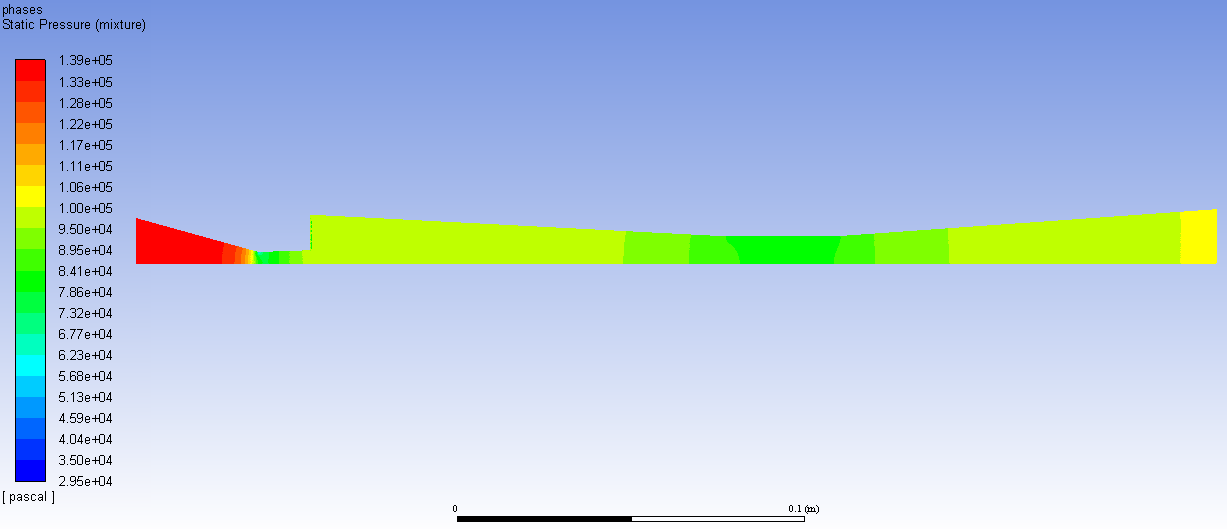
\includegraphics[height=5cm]{images/PressureContour.PNG}
    \end{figure}
\end{frame}

\begin{frame}{Pressure Plot on Steam Central Jet}
   \begin{figure}
    \centering
    \label{fig:pressureplot}
    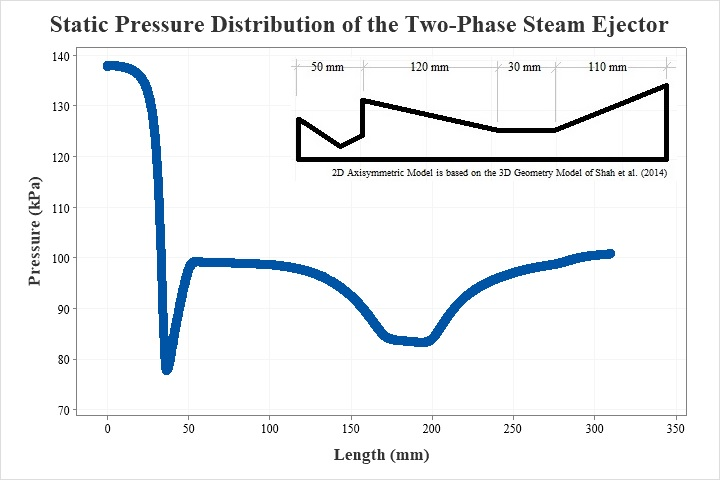
\includegraphics[height=5cm]{images/PressurePlot.jpg}
   \end{figure}
\end{frame}

\begin{frame}{Velocity Contours on Steam Central Jet}
    \begin{figure}
        \centering
        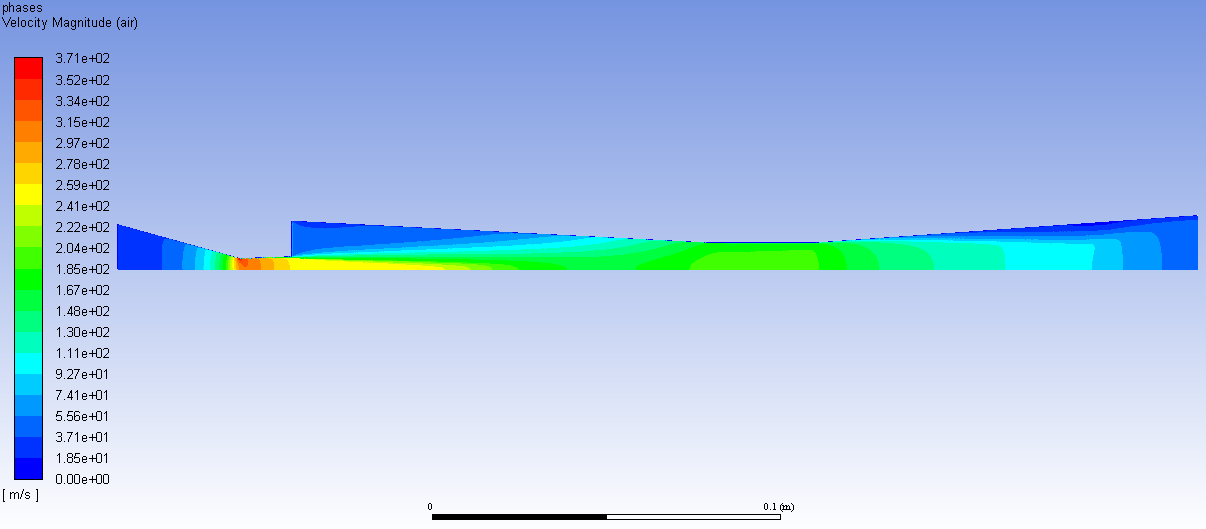
\includegraphics[height=5cm]{images/sjcentralairvel.png}
    \end{figure}
\end{frame}

\begin{frame}{Velocity Contours on Steam Central Jet}
    \begin{figure}
        \centering
        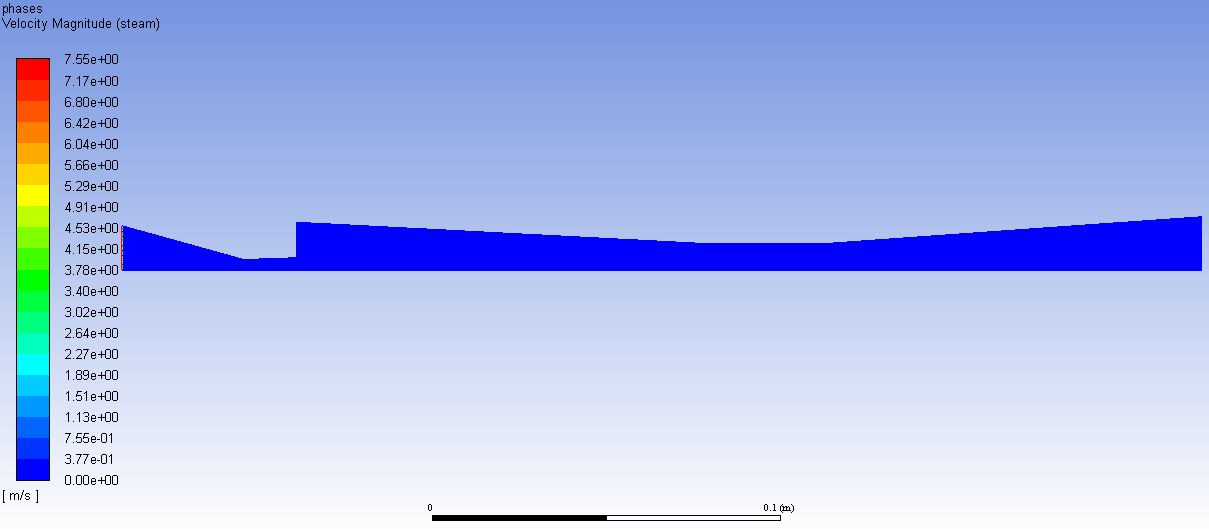
\includegraphics[height=5cm]{images/sjcentralsteamvel.png}
    \end{figure}
\end{frame}

\begin{frame}{Velocity Contours on Steam Central Jet}
    \begin{figure}
        \centering
        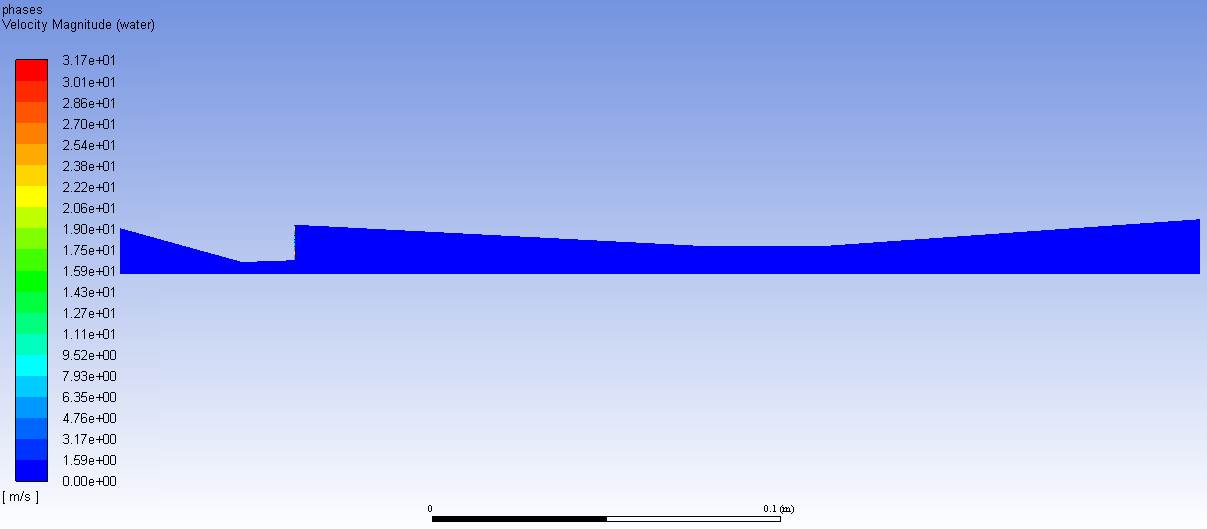
\includegraphics[height=5cm]{images/sjcentralwatervel.png}
    \end{figure}
\end{frame}

\begin{frame}{XY Plots on Steam Central Jet}
  \begin{columns}
   \column{0.45\textwidth}
   \begin{figure}
    \centering
    \label{fig:velocityplot}
    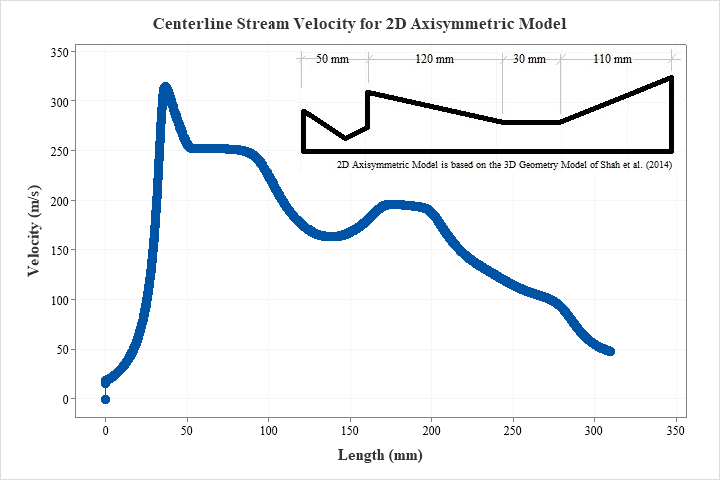
\includegraphics[height=4.5cm]{images/velocityplotcorrect.png}
   \end{figure}
   \column{0.45\textwidth}
   \begin{figure}
        \centering
        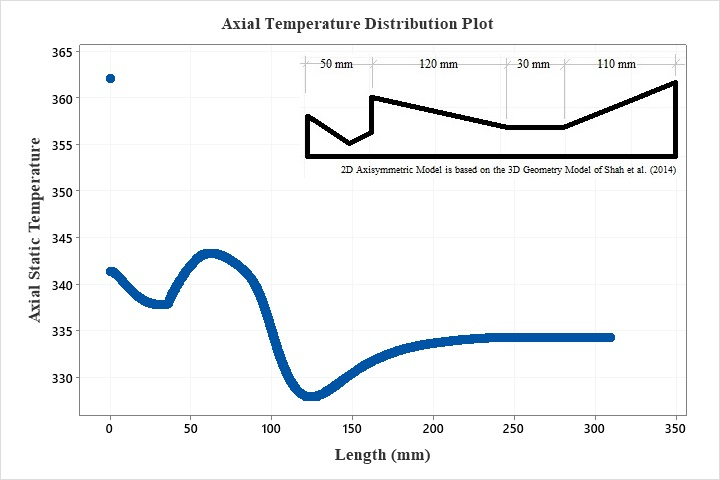
\includegraphics[height=4.5cm]{images/temperatureprofile.jpg}
        \label{fig:axial temperature plot}
    \end{figure}
  \end{columns}
\end{frame}

\begin{frame}{Y Plus on Steam Central Jet}
  \begin{columns}
   \column{0.45\textwidth}
   \begin{figure}
    \centering
    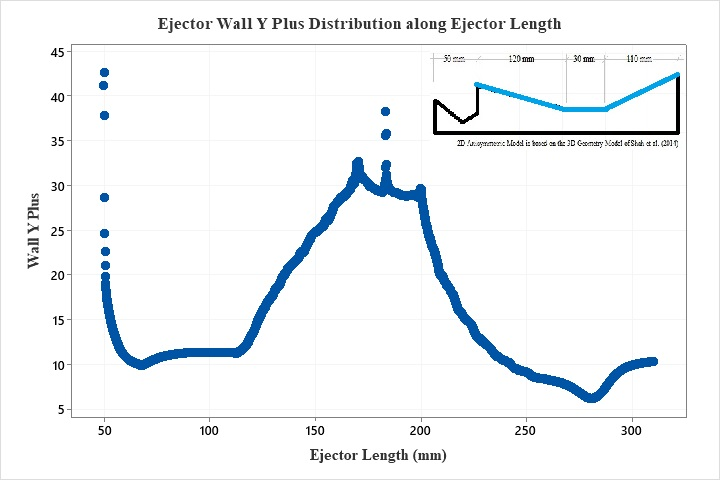
\includegraphics[height=4.5cm]{images/EjectorWallYplus.jpg}
   \end{figure}
   \column{0.45\textwidth}
   \begin{figure}
    \centering
    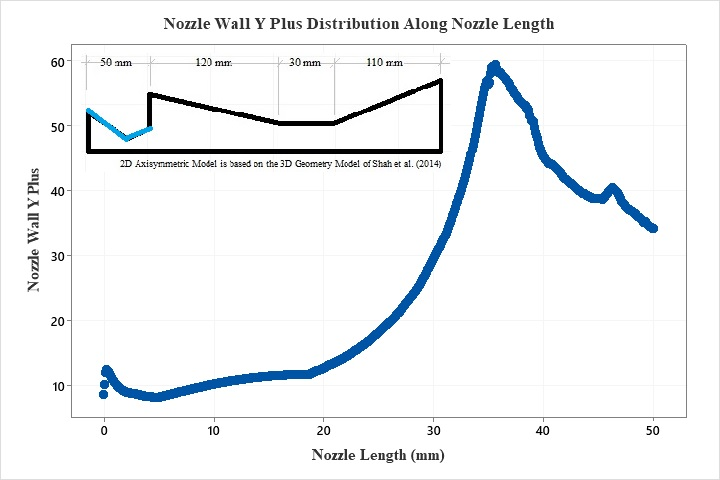
\includegraphics[height=4.5cm]{images/nozzlewallyplus.jpg}
   \end{figure}
  \end{columns}
\end{frame}

\begin{frame}{Water Central Jet: Pressure Plot}
   \begin{columns}
   \column{0.45\textwidth}
   \begin{figure}
    \centering
    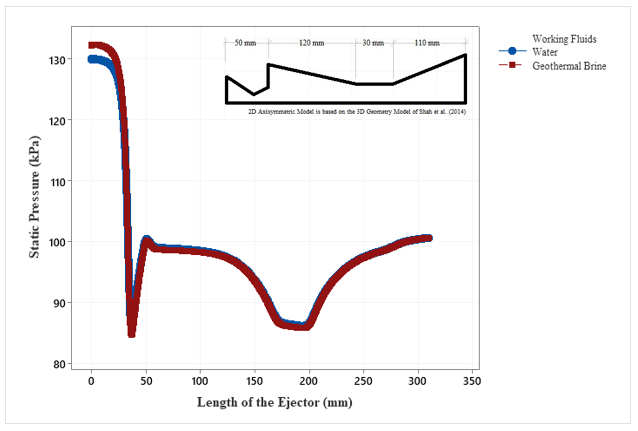
\includegraphics[height=4.5cm]{images/wcwfluids.png}
   \end{figure}
   \column{0.45\textwidth}
   \begin{figure}
    \centering
    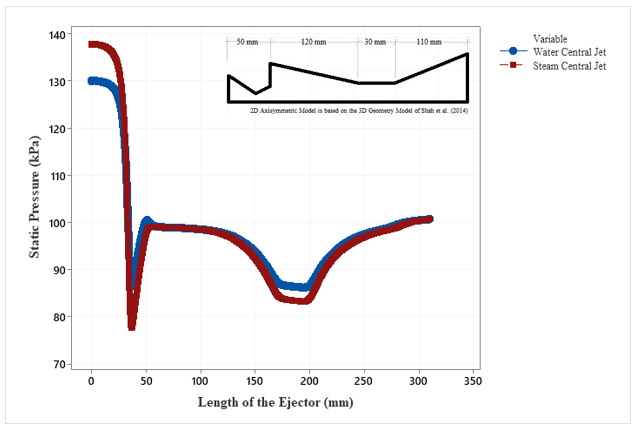
\includegraphics[height=4.5cm]{images/wcandsc.png}
   \end{figure}
  \end{columns}
\end{frame}

\begin{frame}{Water Central Jet: Pressure Contour}
    \begin{figure}
        \centering
        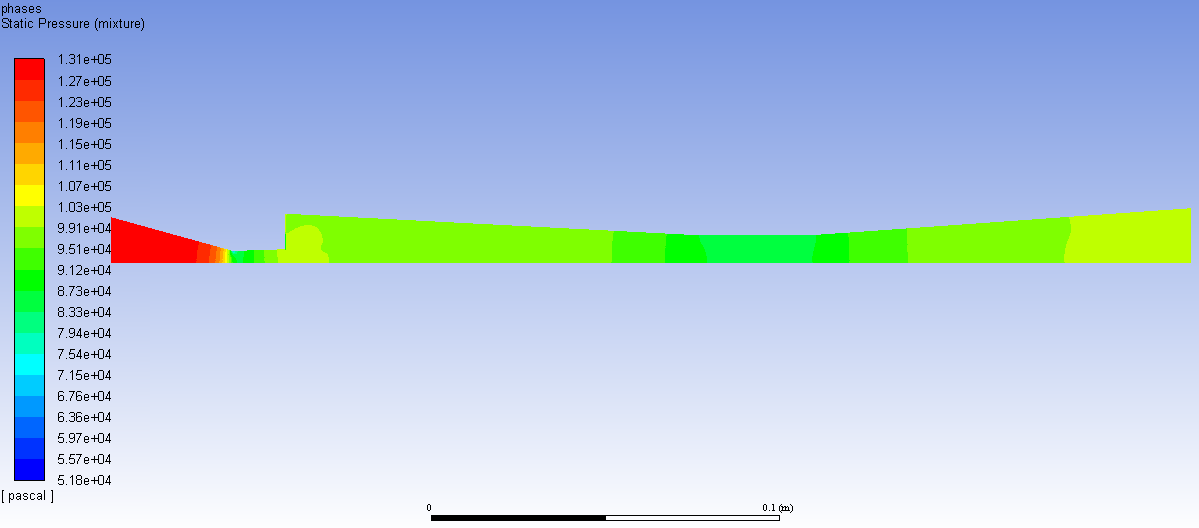
\includegraphics[height=4.25cm]{images/wcpressureplot.png}
    \end{figure}
\end{frame}

\begin{frame}{Water Central Jet: Velocity Plot}
    \begin{figure}
        \centering
        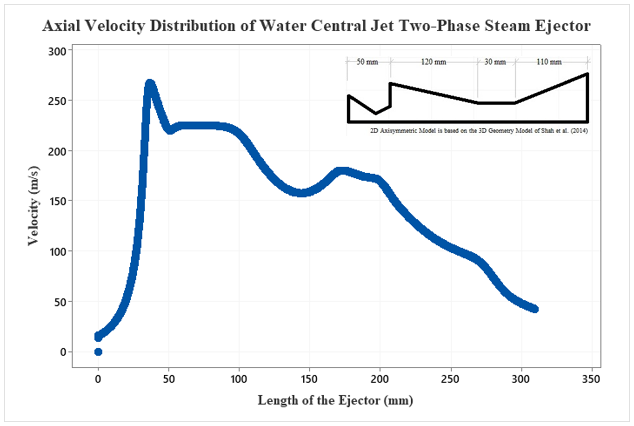
\includegraphics[height=5.5cm]{images/wcjetvelocity.png}
    \end{figure}
\end{frame}

\begin{frame}{Water Central Jet: Velocity Contours}
    \begin{figure}
        \centering
        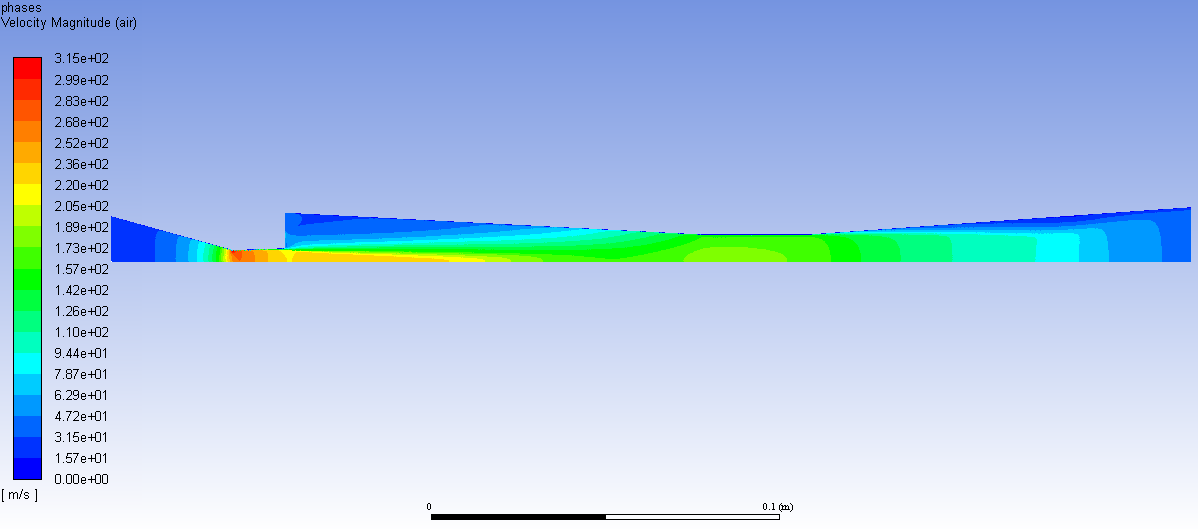
\includegraphics[height=5.5cm]{images/wcvelocityair.png}
    \end{figure}
\end{frame}

\begin{frame}{Water Central Jet: Velocity Contours}
    \begin{figure}
        \centering
        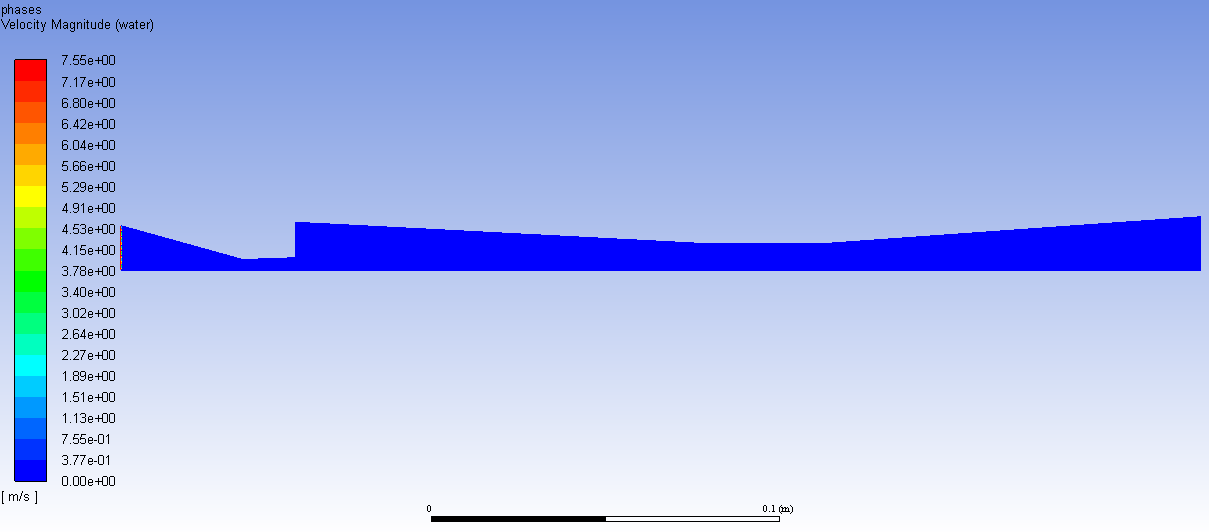
\includegraphics[height=5.5cm]{images/wcjetwatervelcon.png}
    \end{figure}
\end{frame}

\begin{frame}{Water Central Jet: Velocity Contours}
    \begin{figure}
        \centering
        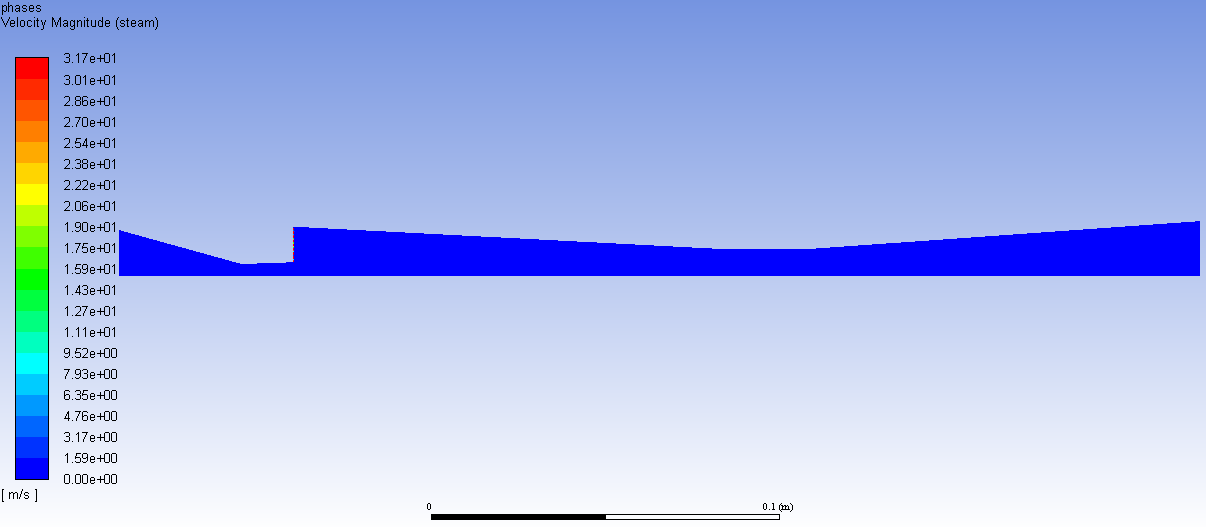
\includegraphics[height=5.5cm]{images/wcjetsteamvelcon.png}
    \end{figure}
\end{frame}

\begin{frame}{Water Central Jet: Axial Temperature Distribution}
    \begin{figure}
        \centering
        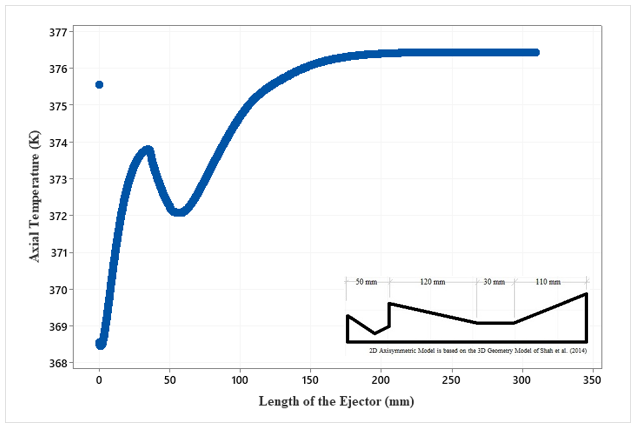
\includegraphics[height=5.5cm]{images/wcjetaxialtemp.png}
    \end{figure}
\end{frame}

\begin{frame}{Y Plus on Water Central Jet}
  \begin{columns}
    \column{0.45\textwidth}
    \begin{figure}
        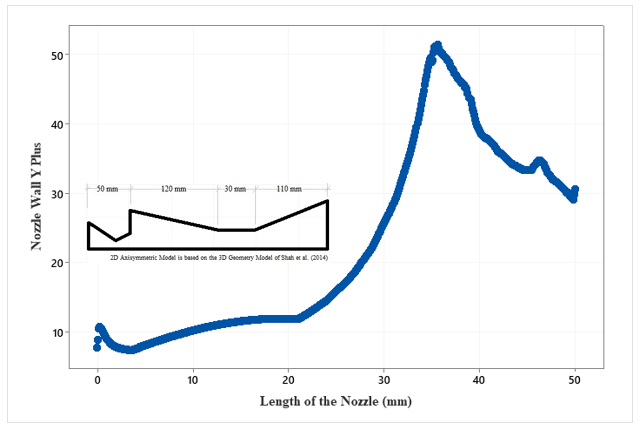
\includegraphics[height=4.5cm]{images/wcjetnozyplus.png}
    \end{figure}
    \column{0.45\textwidth}
    \begin{figure}
        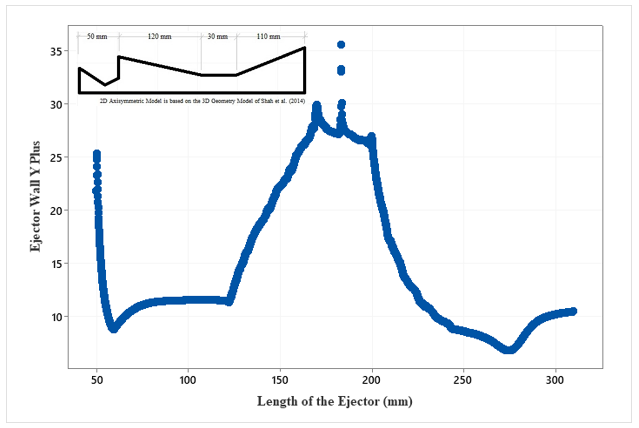
\includegraphics[height=4.5cm]{images/wcjetejecyplus.png}
    \end{figure}
  \end{columns}
\end{frame}

\begin{frame}{Partial Evaporation of Water Central Jet:20\% vapor quality}
\begin{columns}
    \column{0.45\textwidth}
        \begin{figure}
        \centering
        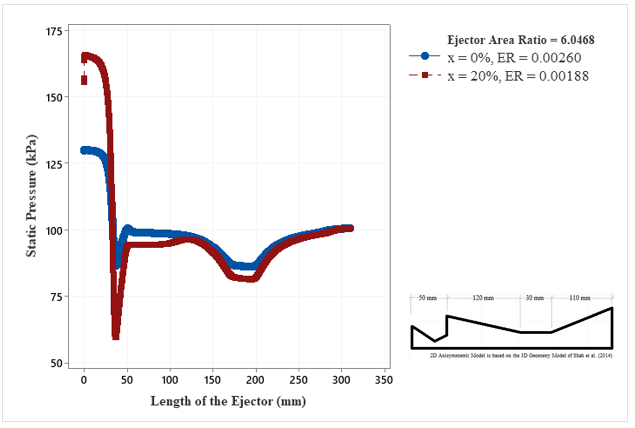
\includegraphics[height=4.5cm]{images/partialevap20percent.png}
    \end{figure}
    \column{0.45\textwidth}
        \begin{figure}
        \centering
        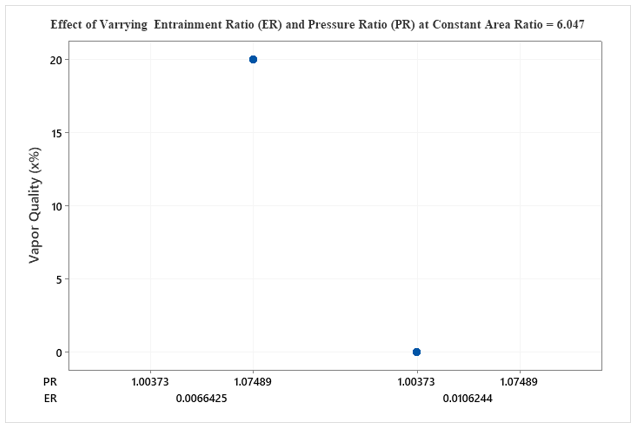
\includegraphics[height=4.5cm]{images/pevaperprinitial1.png}
    \end{figure}
\end{columns}
\end{frame}

\begin{frame}{Partial Evaporation of Water Central Jet:20\% vapor quality}
\begin{columns}
    \column{0.45\textwidth}
        \begin{figure}
        \centering
        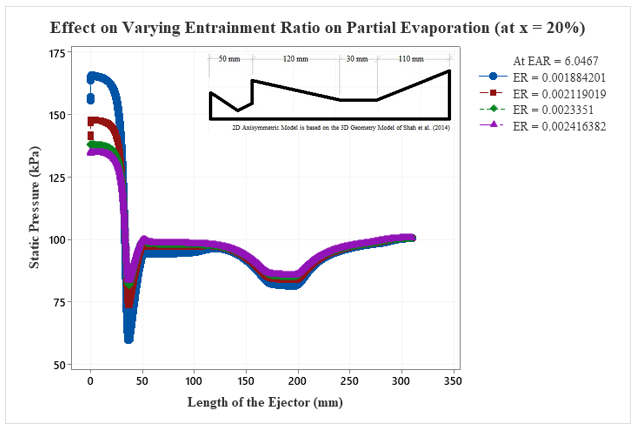
\includegraphics[height=4.5cm]{images/pe20vqver.png}
    \end{figure}
    \column{0.45\textwidth}
        \begin{figure}
        \centering
        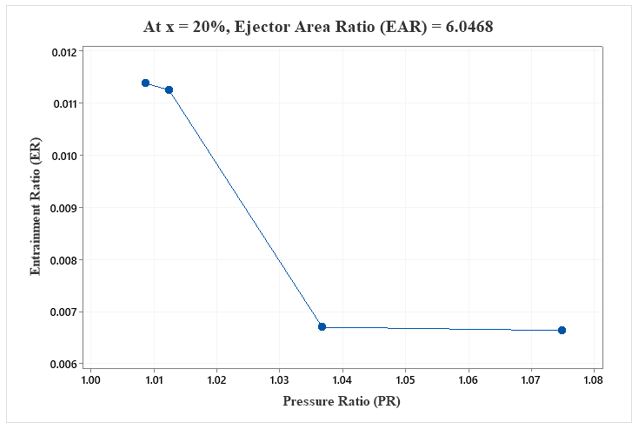
\includegraphics[height=4.5cm]{images/pe20vqerpr.png}
    \end{figure}
\end{columns}
\end{frame}

\begin{frame}{Partial Evaporation of Water Central Jet:20\% vapor quality}
  \begin{columns}
    \column{0.45\textwidth}
    \begin{figure}
        \centering
        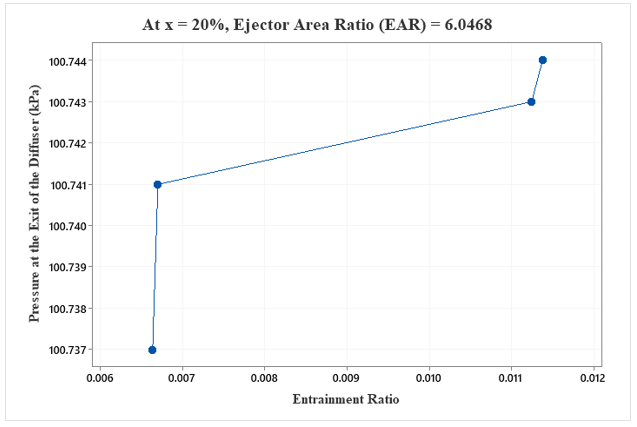
\includegraphics[height=4.5cm]{images/pe20vqpdvser.png}
    \end{figure}
    \column{0.45\textwidth}
    \begin{figure}
        \centering
        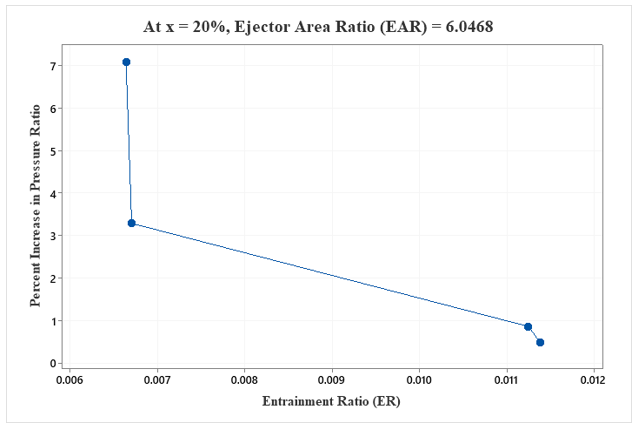
\includegraphics[height=4.5cm]{images/pe20vqpercentincpr.png}
    \end{figure}
  \end{columns}
\end{frame}

\begin{frame}{Initial Findings of the Study}
    \begin{itemize}
        \item The Water Central Jet has pressure drop along the entry of the nozzle and throat mixing area because of the effects of cavitation.
        \item On the Effects of Partial Evaporation, the introducing of vapor to the motive fluid increases the pressure recovery (i.e. pressure ratio) of the ejector, however, further increasing the Entrainment Ratio leads to decrease of pressure recovery because of the pressure drift loss of the secondary fluid to the induced vapor of the motive steam.
    \end{itemize}
\end{frame}

\begin{frame}{Expectations from the Completion of this Research}
    \begin{itemize}
        \item Comprehensive Characterization of the Ejector thru its sensitivity analysis by varying its Ejector Area Ratio, Entrainment Ratio, and Vapor Quality.
        \item Conduct Thermodynamic Analysis to the NOHTFPECGPPIE, this includes exergy analysis, UA analysis, etc.
    \end{itemize}
\end{frame}